\section{Tierra Pirata}

\subsection{Mapa y manejo de memoria}

La memoria se va a distribuir la siguiente manera:

\begin{figure}[H]
	\begin{center}
		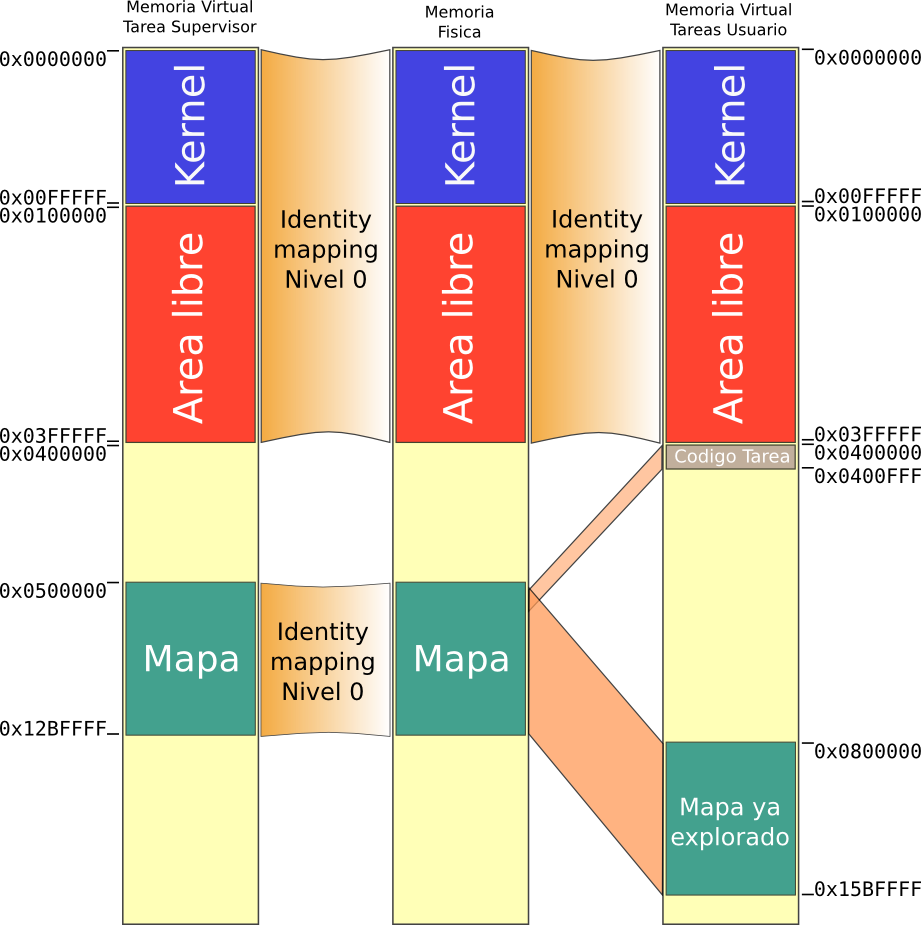
\includegraphics[scale=0.45]{images/MemoriaVirtual.png}
		\caption{Organización de la Memoria.}
		\label{fig:memoria}
	\end{center}
\end{figure}

La Directory Table del kernel tendrá paginado todo lo útil de la memoria en identity mapping.

Luego cada tarea pirata va a tener su propia Directory Table donde se van a paginar los primeros 4MB de memoria en modo supervisor, luego el código de la tarea, que se encontrara en una posición del mapa, sera mapeado a la dirección virtual 0x400000 en modo user y con derechos de escritura; por ultimo se mapeara el mapa a la posición 0x800000, solo paginando las posiciones ya exploradas por el jugador en modo user con derechos de solo lectura.

Las Directory Tables de las tareas se localizaran dentro del área libre de la memoria, como se ve en la figura 12.

Escribimos funciones de inicialización tanto para la memoria virtual del kernel como para la memoria virtual de los piratas, las siguientes funciones deben ser llamadas en el proceso de inicialización de ambos:

\begin{itemize}
\item \fun{void mmu\_inicializar\_dir\_kernel()}: se ocupa de hacer el identity mapping de 4MB del kernel. Además, le mapea todo el mapa en modo escritura, lo que nos permitirá a futuro manejar todo el movimiento de los piratas.

\item \fun{int mmu\_inicializar\_dir\_pirata(uint directoryBase, uint pirateCodeBaseSrc, uint pirateCodeBaseDst)}: Se encarga de realizar el identity mapping de los primeros 4MB de memoria física, los cuales incluyen 
\end{itemize}

Hay que tener en cuenta que para poder hacer el correcto funcionamiento del sistema hay que tener lugar asignado para las pilas, tanto de nivel usuario como de nivel 0, ya que al estar ejecutando una tarea, si se recibe una interrupción tanto interna, de software o externa, el estado del sistema pasara a nivel 0, por lo tanto se necesitara una pila separada de nivel 0.

Por lo tanto la decisión que tomamos tener una pagina (dentro del área libre) por cada tarea pirata, donde colocaremos la pila de nivel 0. Y la pila de nivel usuario se colocara al final de la pagina donde se encuentra su código. En la figura 12 se ve la localización de las pilas de nivel 0 de las tareas pirata.

Con respecto a la necesidad de tener que pedir espacio paginas memoria donde ir colocando las Page Tables para todo el sistema de paginación, ya sean tareas piratas o kernel, vamos a asignándolas en el área libre a medida que sean pedidas, organizándolas como muestra la figura 12.

\begin{figure}[H]
	\begin{center}
		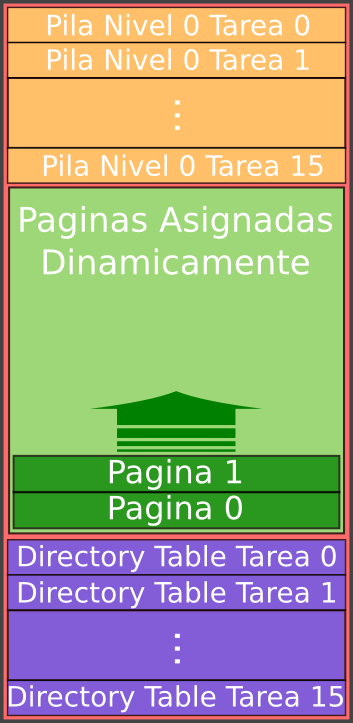
\includegraphics[scale=0.45]{images/AreaLibre.png}
		\caption{Organización del área libre.}
		\label{fig:arealibre}
	\end{center}
\end{figure}

\subsection{Manejo de interrupciones}

\subsubsection{Reloj}

La interrupción de reloj comienza llamando la función \fun{scheduler\_tick}, que se ocupa de devolver el índice de la tarea en la \texttt{GDT} al que se debe ir. En caso de que se tenga que intercambiar de tarea, la rutina de atención de esta interrupción hace un \texttt{jump far} a la nueva tarea.

\subsubsection{Teclado}

Cuando hay una interrupción de teclado, la tecla que ha sido presionada se codifica con un \texttt{scan code} de 8 bits, que se guarda en el controlador de teclado. Estas se leen a través del puerto \hex{0x60} con la instrucción \texttt{in al, 0x60}. Una vez guardado el código, se llama a la función de C \fun{isr\_keyboard}, a la que se le pasa el código por pila respetando la convención C de 32 bits.

La función \fun{isr\_keyboard} luego le asigna diferentes funciones a las teclas \texttt{right\_shift}, \texttt{left\_shift} e \texttt{y}. Todos los scan codes están definidos en \texttt{keyboardcodes.h}.

\subsubsection{Syscall}
El sistema provee un servicio a las diferentes tareas mediante la interrupción \hex{0x46}. La misma le permite a las tareas usar de forma indirecta las siguientes funciones.
\begin{enumerate}
\item \fun{game\_syscall\_pirata\_mover}: Mueve al pirata de una posición a otra. Si el pirata que llamo a esta función es un minero, requiere que la pagina a la que  se quiere mover ya este paginada. Al moverse el pirata, también se mueve su código, y se debe también remappear la dirección \addr{0x400000} a la nueva dirección física donde el código se ha movido.

Si un pirata explorador al moverse encuentra un tesoro, se lanza un pirata minero automáticamente. Al mismo se le debe pasar la posición del tesoro por parámetro. Utilizando la convención C y el stack correspondiente a la nueva tarea, escribimos los parámetros en el stack de la dirección física de su respectivo codigo.

Cuando programamos esto tuvimos el siguiente problema. La interrupción al mover causaba un escalamiento de privilegios, pero seguíamos manteniendo el \reg{cr3} de la tarea que encontró el tesoro. Por esta razón no podíamos escribir en el stack de la nueva tarea y teníamos un \#GP Fault. Esto se debe a que las tareas tienen paginadas la memoria en solo lectura. Para resolver esto, simplemente cambiamos el \reg{cr3} por el del kernel antes de escribir en el stack y luego lo restauramos.

\item \fun{game\_syscall\_cavar}: Actualiza los puntajes y los atributos del tesoro correspondiente cuando un pirata minero cava. En caso de que se acaben las monedas del tesoro, el pirata se desaloja con la función \fun{game\_pirata\_exploto}
\item \fun{game\_syscall\_pirata\_posicion}: Devuelve la posición del pirata. La misma se codifica como y $<<$ 8 $|$ x en un entero.
\end{enumerate}

El Syscall se llama indirectamente a través de \texttt{inline asm}, que se ocupa de pasar los parámetros y llamar a la respectiva función. Al ejecutar esta interrupción hay un escalamiento de privilegios a nivel 0, lo que permite manipular la memoria y ejecutar funciones que no se podrían ejecutar desde una tarea (user), como por ejemplo manipular los directorios de pagina.

\subsection{Scheduler}

El Scheduler es una función en C que es llamada por la interrupción de teclado. La misma de identificar la tarea que se debe ejecutar actualmente para respetar el siguiente diagrama:

\begin{figure}[H]
  \centering
    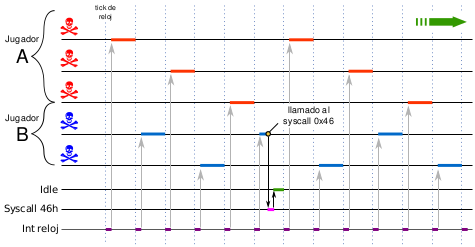
\includegraphics[width=0.7\textwidth]{images/scheduler}
  \caption{Diagrama de Tareas}
\end{figure}

El algorítmo de scheduling funciona, a grosso modo (en el código fuente hay comentarios explicandolo más en detalle) manteniendo en todo momento el índice del próximo pirata que debería jugar (tanto para el jugador A como el B), el índice del próximo jugador a ejecutarse, y la cantidad de ticks de timer que lleva (estos ticks se resetean cada \texttt{SCHEDULER\_TASK\_TICKS} interrupciones, y se incrementa cada vez que el timer interrumpe). Entonces, cuando los ticks del timer se vuelven 0, recorre para el jugador correspondiente todas las tareas empezando del índice denotado, hasta alcanzar de vuelta este valor. Si encuentra una tarea existente, la ejecuta, en caso contrario, intenta con el otro jugador. Suponiendo que no encuentre ninguna tarea a ejecutar, termina haciendo el switch a la Idle. Es importante notar que no hacemos task switch si la próxima tarea a ejecutar es igual a la que se está ejecutando, o si el valor de retorno del scheduler no es -1 (esto va a suceder siempre que el contador de ticks no esté en el estado inicial).

Además, cada vez que tenemos una interrupción por software terminamos saltando a la Idle por el resto del quantum de tiempo que le corresponde a la tarea.

\subsection{Estructuras}

Para mantener cuenta del estado del juego y de cada uno de los jugadores, creamos algunas estructuras definidas en \texttt{game.h}. Para saber que posiciones del mapa ya han sido paginadas, cada jugador mantiene un \texttt{bit\_map} con (\texttt{MAPA\_ALTO} * \texttt{MAPA\_ANCHO} / 8) chars. Cada bit corresponde a una pagina del mapa. De esta manera, al lanzar un pirata podemos saber muy fácilmente qué páginas le debemos mapear.
 de la 